\chapter[The Properties of Reconnection Current Sheets in GRMHD Simulations of Radiatively Inefficient Accretion Flows]
{The Properties of Reconnection Current Sheets in GRMHD Simulations of Radiatively Inefficient Accretion Flows}

\section{Introduction}
In this chapter, we use representative GRMHD simulations to assess whether reconnection regions frequently
occur in global simulations. We consider simulations
with Standard and Normal Evolution (SANE) and Magnetically Arrested Disk (MAD) initial magnetic field configurations (e.g., \citealt{narayan2012}). In the SANE case, the magnetic field is initialized with alternating poloidal loops, while the MAD initial field consists of a single poloidal loop, which results
in the magnetic field playing a more dominant role in
the dynamics of the disk. We devise criteria to locate
regions of field reversal and characterize the properties
of the plasma in these regions. We focus on the plasma-$\beta$
and magnetization parameter $\sigma$, which have been shown
to play an important role in particle acceleration. We
also identify field components that are orthogonal to
the reversing field, often referred to as guide fields, and
quantify their strengths. Our results will guide future
particle-in-cell (PIC) studies of low-luminosity accretion
flows. Finally, we compute the time-dependent magnetic
energy available in reconnection regions to assess whether
this is a plausible mechanism to generate the observed Xray variability of Sgr A*.

\section{Characterizing Potential Reconnection Regions in MHD Simulations}
Magnetic reconnection takes place in regions where
there is a reversal of magnetic field over a short characteristic length scale, in which the current density becomes large. In typical simulations of the local dynamics
of reconnection, the initial condition is specified in terms
of a Harris sheet, which has the magnetic field profile

\begin{equation}
	\bold{B} = B_0 \tanh{\frac{x}{L}}\hat{y}
\end{equation}

In this geometry, the y-component of the magnetic field
reverses direction over a characteristic length L in the
x-direction. This field reversal has a high curl associated
with it, leading to a sudden peak in the current density,
which scales as
\begin{equation}
	\bold{J}= \frac{B_0}{L}\rm{sech}^2\frac{x}{L}\hat{z}.
\end{equation}

There are only a small number of parameters that determine the particle heating and acceleration that results from reconnection events.  These are the magnetization parameter

\begin{equation}
	\sigma \equiv \frac{B^2}{4 \pi \rho c^2}
\end{equation}

which is the ratio of magnetic energy density to rest mass energy density, and the plasma-$\beta$ parameter

\begin{equation}
	\beta \equiv \frac{P_{\rm{gas}}}{P_{\rm{magnetic}}}=\frac{8\pi n k T}{B^2},
\end{equation} 

which specifies the ratio of gas pressure to magnetic pressure.  Here, $\rho$, $n$, and $T$ are the mass density, number density, and temperature of the plasma particles, respectively.

Another important quantity to consider for magnetic
reconnection is the magnitude and direction, if present,
of the so-called guide field. This is the component of the
magnetic field in the sheet perpendicular to the reconnecting field. The effect of such a guide field on particle
acceleration has been studied in certain regimes (\citealt{wang2016, dahlin2016, stanier2016}) and, in
some cases, can have an effect on the resulting electron
energy distribution.
Our first goal is to devise an algorithm that will allow
us to identify the location and relevant properties of potential reconnection regions, i.e., Harris sheets, in global
GRMHD simulations, which we describe in the following


\section{Finding and characterizing current sheets}
As an illustrative example, we use two 60 hr (about
$11,000 \; GM/c^3$
) long GRMHD simulations of a radiatively inefficient accretion flow onto a black hole
(\citealt{narayan2012}) that were
performed using the HARM code (\citealt{gammie2003}).
These simulations were employed in a large study of the
broadband, time-dependent emission from Sgr A* (\citealt{chan2015a,chan2015b}) where we coupled HARM to the radiative
transfer algorithm GRay (\citealt{chan2013}) and varied
the black hole spin, density normalization, observer inclination, initial magnetic field configuration, as well as
the electron thermodynamic prescription. From these
investigations, we identified 5 models that best fit the
steady-state broadband spectrum as well as the previously observed 1.3 mm image size of Sgr A* and also
characterized their variability properties. In the present
study, we use two representative models from \citet{chan2015b}: a SANE model with a black hole spin a = 0.7
and a MAD model with a black hole spin a = 0.9. In general, the thermal SANE models tend to show short-lived,
high amplitude variability in their IR and mm flux, while
the thermal MAD models tend to show lightcurves dominated by smooth and long-timescale flux changes.
Our goal is to identify in each snapshot from these simulations potential regions of reconnection. Because of the
large shear in the accretion flow, the magnetic fields are
primarily toroidal and the alternating components occur
primarily in the azimuthal direction. For this reason,
we search through the simulation volume for cells that
have both a high current relative to the mean value in
the snapshot as well as very low values of the azimuthal
component of the magnetic field $B_{\phi}$ in order to pick out
the sheets where reconnection may occur.
Specifically, we consider 2D slices of the simulation volume at each azimuthal angle $\phi$ at each snapshot and identify the points that (i) have current magnitudes $\sqrt{J_\mu J^\mu}$
that are higher than four times the mean current of that
snapshot and (ii) $\phi$-components of the magnetic field
smaller than a fiducial value, characterized by the usual
magnetization parameter $\sigma_\phi = B^2_{\phi}/(4 \pi m n c^2)$. We use a
$\sigma_\phi$ threshold of $10^{-6}$. We then apply an algorithm similar to the one described in \citet{zhdankin2013} for
identifying and analyzing the statistics of current sheets
in shearing box simulations of MHD turbulence. For every point with grid indices ($i$, $j$) on an azimuthal slice of
our domain picked out by the above criteria with current
magnitude $J_{\rm{peak}}$, we consider all 4 adjacent points in the
grid. If the current at an adjacent point is above $J_{\rm{peak}}/2$,
while also satisfying $\sigma_{\phi}<10^{-6}$
, we consider it as part
of the same current sheet. We continue this process of
scanning every point in the sheet, considering all neighboring points, and applying these criteria to them until
no more points are being added to the sheet.
In the top panel of Figure \ref{bphi_sheet_example}, we show the result of
applying this algorithm on a snapshot of the SANE simulation, with the $B_{\phi}$ configuration shown in the bottom
panel of the same figure. It is evident that the regions
between flux tubes of opposing azimuthal magnetic flux
are effectively picked out. When we repeat this procedure on all adjacent azimuthal slices, we find that the
current sheets show large azimuthal extents throughout
the flow, providing ample surface area for neighboring
flux tubes to reconnect over.  We show in Figure \ref{MAD_snapshot}, a representative
snapshot of the MAD simulation for comparison. We see that
the magnetic field strengths about the current sheet in the MAD
simulation are higher than that in SANE. Additionally, we find
that there is typically less fine structure to the MAD current
sheets; the MAD current sheets tend to consist of one or two
relatively flat sheets, while the SANE current sheets are often
highly curved and twisted into complicated geometries, as
shown in the top panel of Figure \ref{SANE_snapshot}.

\begin{figure}[!h]
\centering
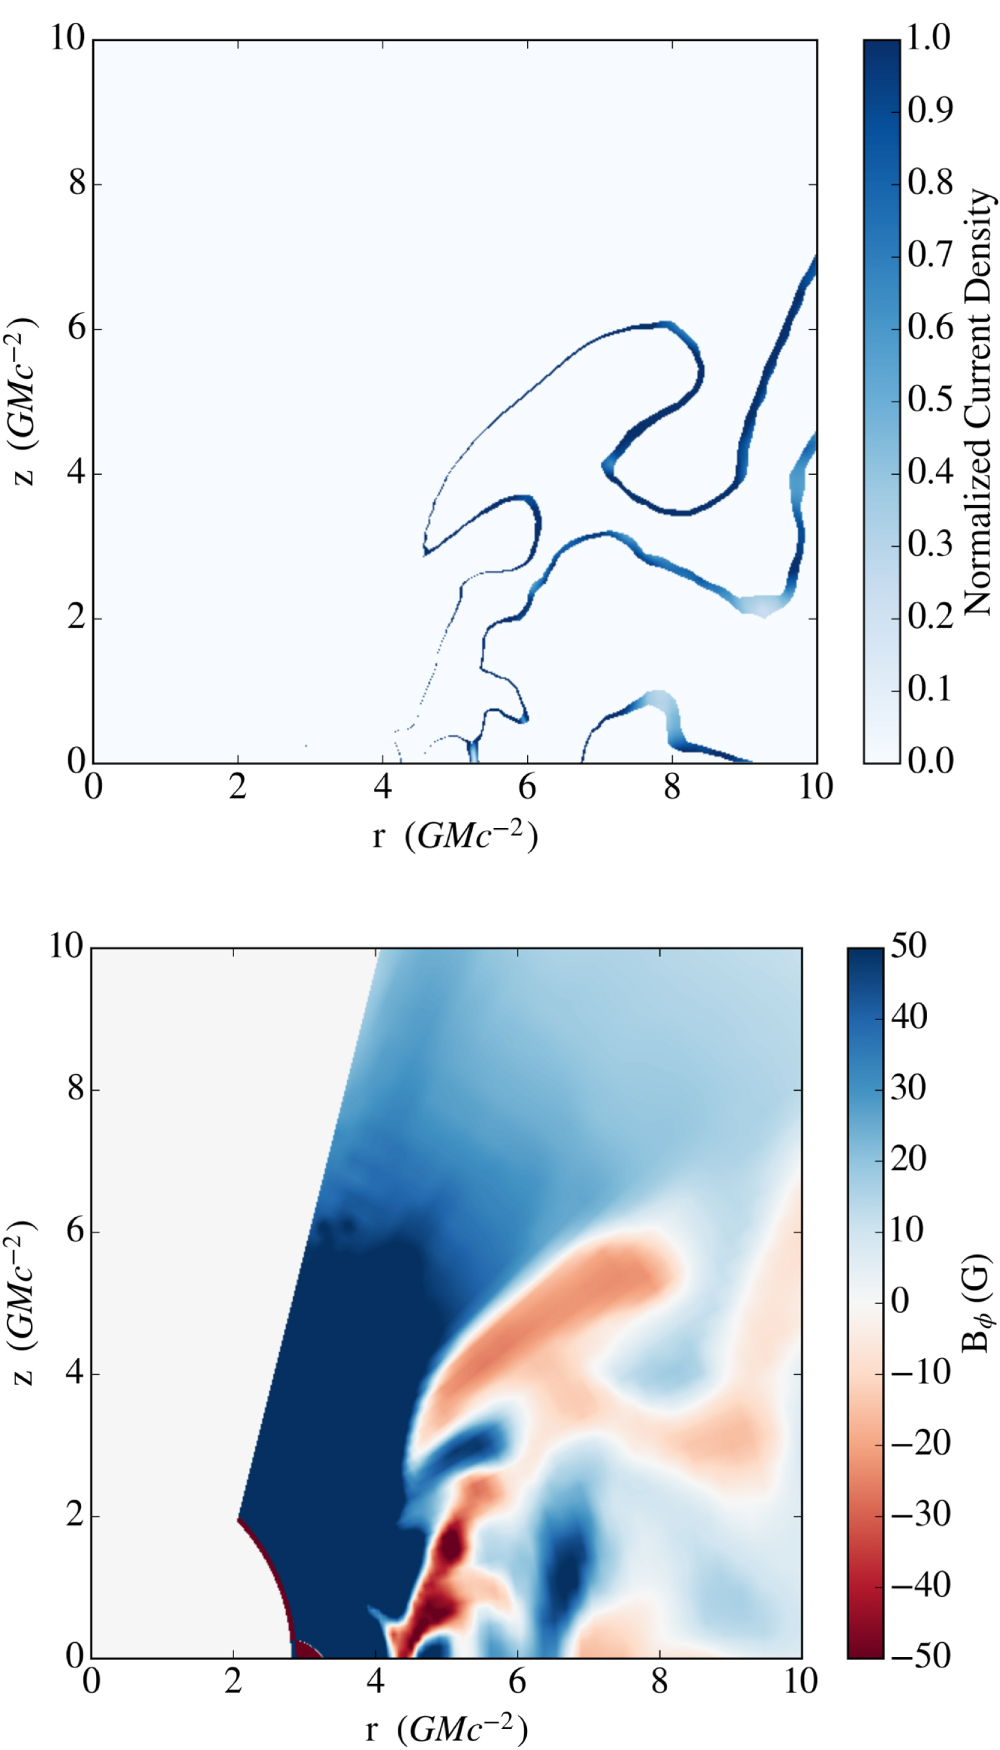
\includegraphics[width =.6\textwidth]{paper2_fig1.jpg}
\caption{(Top) The current sheets picked out by our algorithm in a SANE simulation, at the interface between regions of opposing magnetic flux.  Regions near the pole and within the ISCO are excised to avoid known numerical issues related to the density floor imposed.  (Bottom) A 2D slice of the azimuthal magnetic field in one snapshot of the SANE simulation, showing the presence of numerous opposing flux tubes that provide potential sites of reconnection.}
\label{SANE_snapshot}
\end{figure}


\begin{figure}[!h]
	\centering
	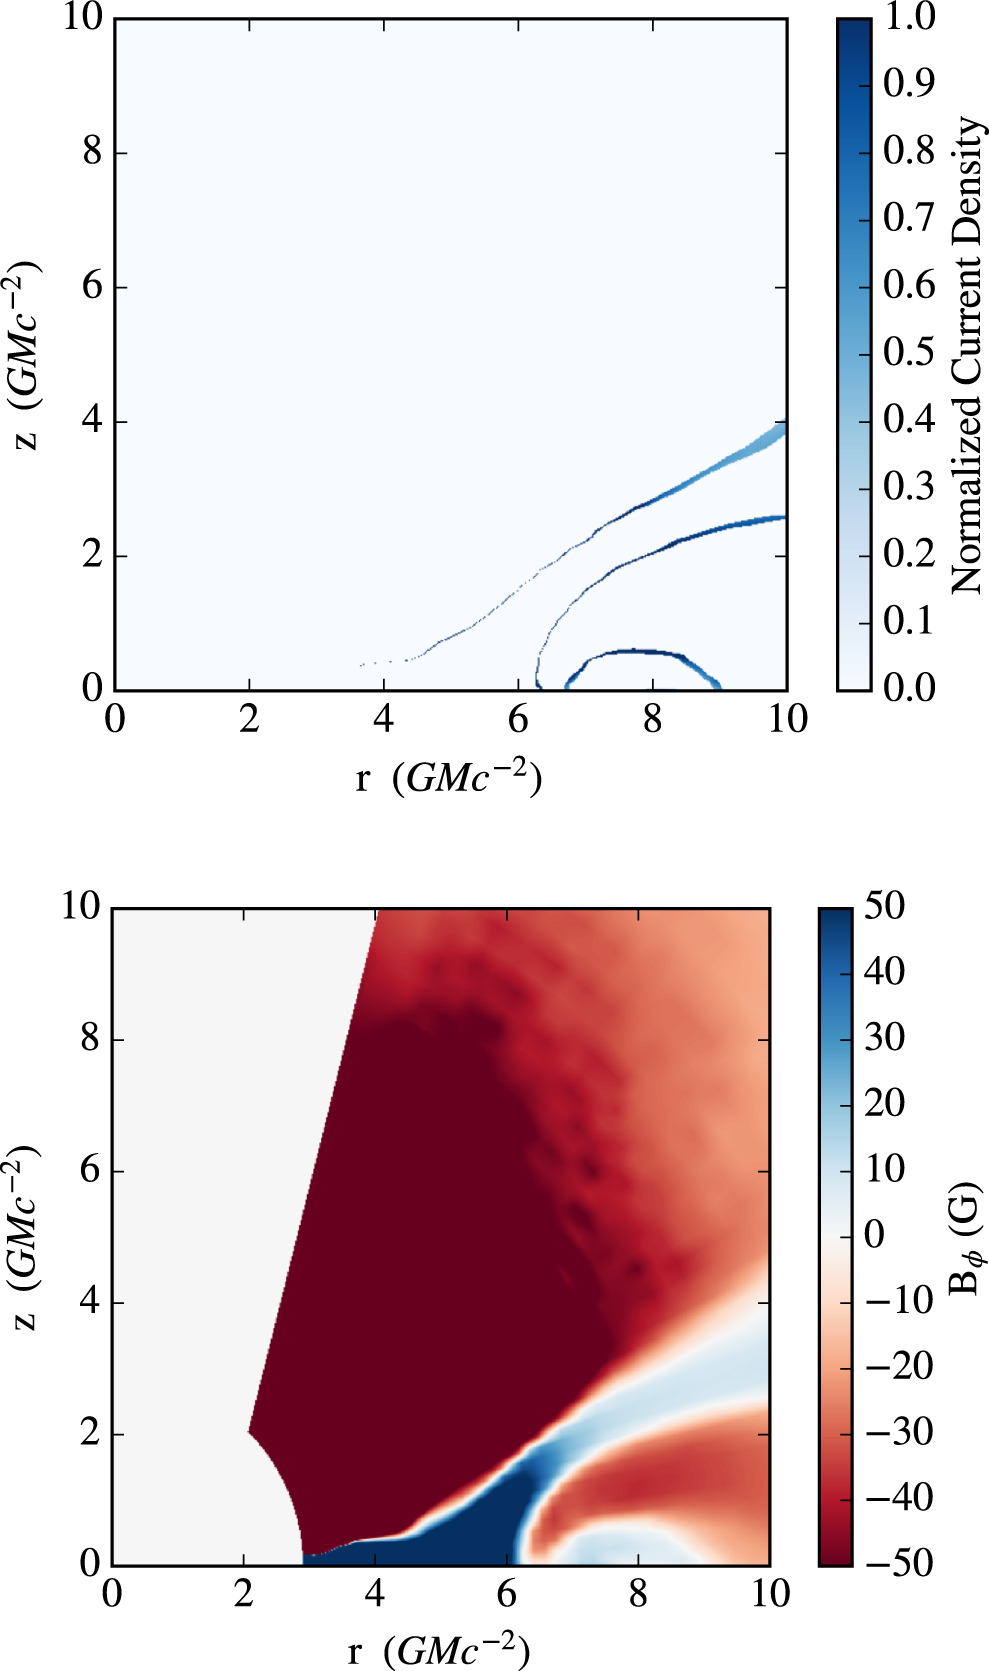
\includegraphics[width =.6\textwidth]{paper2_fig2.jpg}
	\caption{Top: the current sheets picked in a MAD simulation.  Bottom: a 2D slice of the azimuthal magnetic field in one representative snapshot of the MAD simulation.  We see that the typical toroidal field strengths are higher, and that there is generally less structure as compared with the SANE simulation.  We see these difference between SANE and MAD in the majority of snapshots from our simulations.}
	\label{MAD_snapshot}
\end{figure}

\subsection{Sampling Plasma Properties Associated with Current Sheets}
Once we identify the current sheets in each snapshot,
we characterize the plasma parameters of these sheets
that are relevant to magnetic reconnection. The location
that we want to measure these parameters at is not in
the sheet itself but where the magnetic field reaches its
asymptotic value some distance away from the sheet in
a direction perpendicular to it. This breaks down into
two problems: finding the direction perpendicular to the
sheet and determining how far to go along this direction
until the magnetic field reaches its appropriate asymptotic value. 

In order to approximate the direction perpendicular to
the current sheet at a point ($i$, $j$) that has been flagged
as belonging to the sheet, we first find the local slope of
the sheet about this point. To do this, we consider a box
around each point ($i$, $j$) in the sheet, with width $S+1$,
whose corners are at ($i \pm S/2$, $j \pm S/2$). We use a value
of $S = 10$ pixels, which is generally smaller than the
radius of curvature of a current sheet. We then calculate
the slope from the point in the center of this box ($i$, $j$)
to every other point ($i'$, $j'$)
in the box which is flagged
as being part of the current sheet. Taking the inverse
tangent of this slope gives the angle with respect to the
horizontal of the line that passes through ($i$, $j$) and ($i'$,$j'$.
We calculate the average of these angles, approximating
the angle of the current sheet about point ($i$, $j$) as
\begin{equation}
\theta_{mean}=\frac{1}{N}\sum_{\left(i',j'\right)_{1}}^{\left(i',j'\right)_{N}}\arctan{\left[\frac{z(j'_n)-z(j)}{r(i'_{n})-r(i)}\right]}
\end{equation}

We then calculate the mean slope:
\begin{equation}
m_{mean}=\tan{\theta_{mean}}
\end{equation}

and take the direction perpendicular to this slope:

\begin{equation}
m_{\perp}=-\frac{1}{m_{mean}}
\label{meanslope}
\end{equation}

We sample the plasma properties at some distance
along the normal where the toroidal magnetic field has
reached its asymptotic value. We approximate this location by scanning along the normal direction, given by
Equation \ref{meanslope}, until the field profile flattens out. We consider the field sufficiently flat when the fractional change
in magnetic field from one computational cell along the
normal to the next is less than three percent, averaged over two adjacent cells\footnote{Even though the approach outlined here for the definition of orthogonal directions is valid only for a flat spacetime, it is adequate for our present purposes both because we deal with short distances ($\sim 0.1 M$) away from the current sheets and because we are interested in quantifying the typical values of the asymptotic magnetic field without being very sensitive to the precise direction.}

As an illustrative example, Figure \ref{fieldprof} shows the magnetic field
and current density profile along the normal of a current sheet
picked out by our algorithm in the SANE simulation (the
typical shapes of these profiles generalize to the MAD
simulations). We indeed see a Harris-sheet-like structure, with
a magnetic field profile that passes through 0 and asymptotes to
a fixed value at a distance $\approx 0.2-0.3 GMc^{-2}$ away from the
center; the current density has the expected maximum
associated with the steep gradient in magnetic field. To
illustrate the variety of current sheets and show their typical
length scales and field profiles, Figure 4 shows a sample of
current sheets identified in different snapshots and locations of
the SANE simulation. The magnetic field profiles again follow
structures reminiscent of Harris sheets, with the magnetic field
passing in a linear fashion through 0 and reaching an
asymptotic value at a distance that is typically $0.2$ to
$0.6 GMc^{-2}$ away from the center of the sheet. We find that
while the current sheets are often approximately symmetric
(approaching similar magnetic field strengths to either side of
the current sheet), there are also cases of non-symmetric current
sheets, where the asymptotic magnetic field strength differs
between the two sides of the sheet. Studies of magnetic
reconnection almost always employ symmetric current sheets,
but the asymmetry in magnetic field profile could influence the
outcome of reconnection.


\begin{figure}[!h]
	\centering
	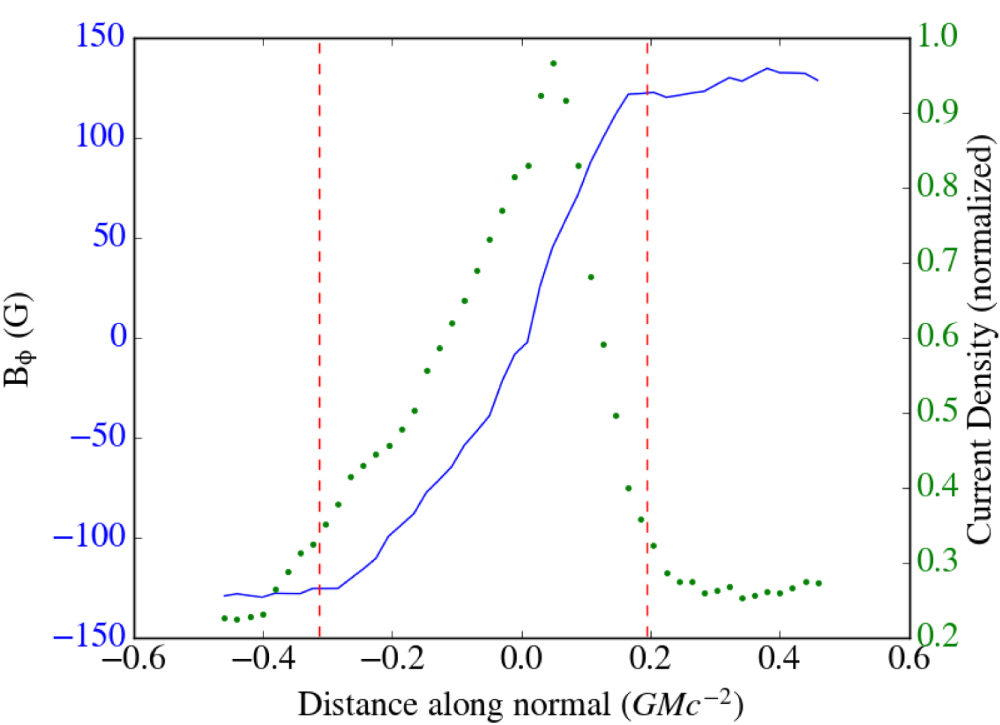
\includegraphics[width =\textwidth]{paper2_fig3.jpg}
	\caption{Magnetic field (blue line) and current density (green points) profiles
		along the normal direction to a current sheet showing the typical field reversal
		across the current sheet and the associated maximum in current density. The
		red dashed lines indicate the location at which we sample the relevant plasma
		parameters.}
	\label{fieldprof}
\end{figure}


\begin{figure}[!h]
	\centering
	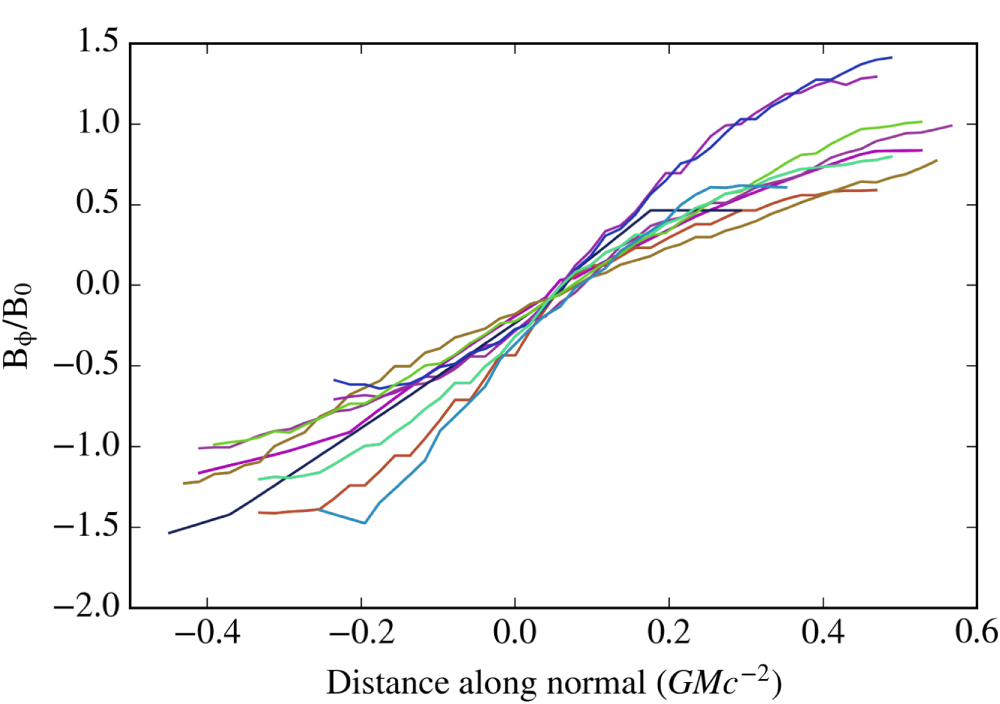
\includegraphics[width =\textwidth]{paper2_fig4.jpg}
	\caption{Random selection of field profiles from the simulation across current
		sheets, showing that the typical behavior is reminiscent of the idealized Harrissheet structure, passing linearly through 0 and asymptoting to similar values on
		either side of the sheet. The vertical scale is normalized to the average
		asymptotic magnetic field for each sheet.}
	\label{many_fieldprof}
\end{figure}

\section{Plasma Properties of Current Sheets}
Having established the frequent occurrence and geometry of potential reconnection regions, our second goal
is to investigate the properties of current sheets in timedependent simulations of accretion flows and characterize
the parameters relevant to non-thermal particle acceleration to inform further PIC studies. We ultimately wish to
determine the role of magnetic reconnection in contributing to the multiwavelength variability of low-luminosity
accretion flows.
Iterating through timesteps in our simulations, we
find the current sheets and, at every point in each sheet,
determine the asymptotic values of $\sigma$ and $\beta$ as well as
the guide field strength at the center of the sheet for
both our SANE and MAD simulations, as described
below.

\subsection{Properties of SANE Current Sheets}
For the SANE simulation, in the regions where reconnection may occur, the magnetization $\sigma$ ranges from $10^{-4}$ to 1, while the plasma-$\beta$ ranges from $0.1$ to $10^3$, as shown in Figure \ref{SANE_hist}
The anticorrelation evident in Figure \ref{SANE_hist} (see also Figure \ref{MAD_hist}) occurs because the magnetization parameter scales as $B^2/n$, while the plasma-$\beta$ scales as $(B^2/n)^{-1}$.  The spread arises because the plasma-$\beta$ also depends on the plasma temperature.



\begin{figure}[!h]
	\centering
	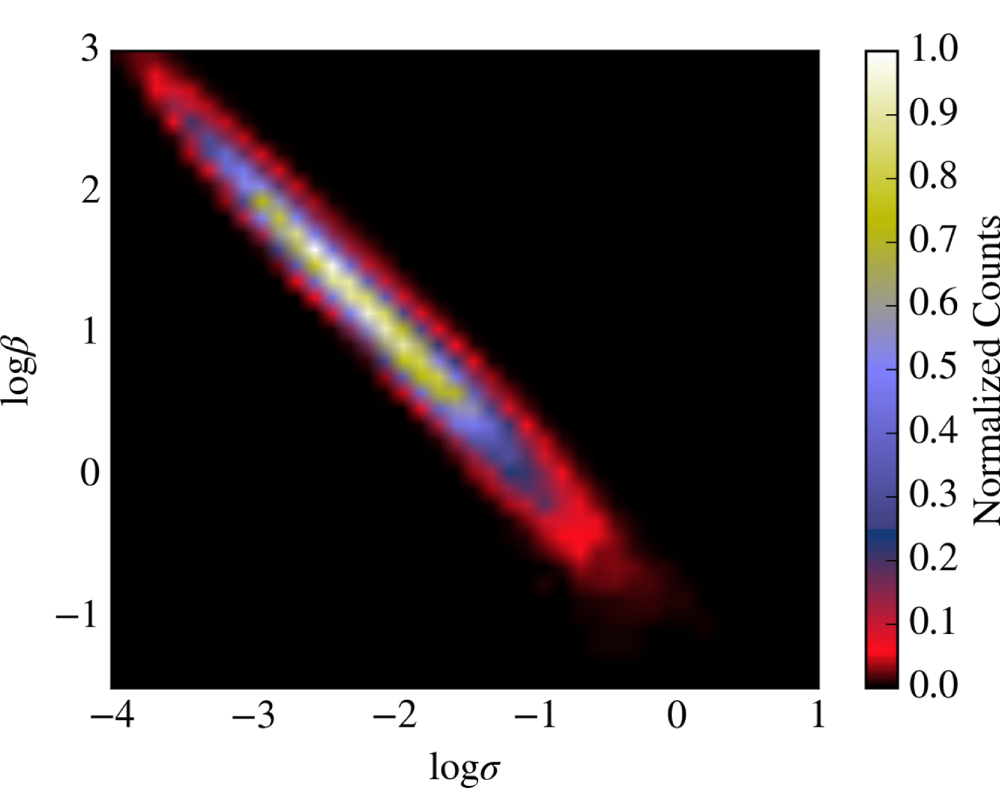
\includegraphics[width =\textwidth]{paper2_fig5.jpg}
	\caption{Two-dimensional histogram of the magnetization $\sigma$ and plasma-$\beta$ across all current sheets in the inner $10 \; GM/c^2$ of the SANE simulation.}
	\label{SANE_hist}
\end{figure}

\begin{figure}[!h]
	\centering
	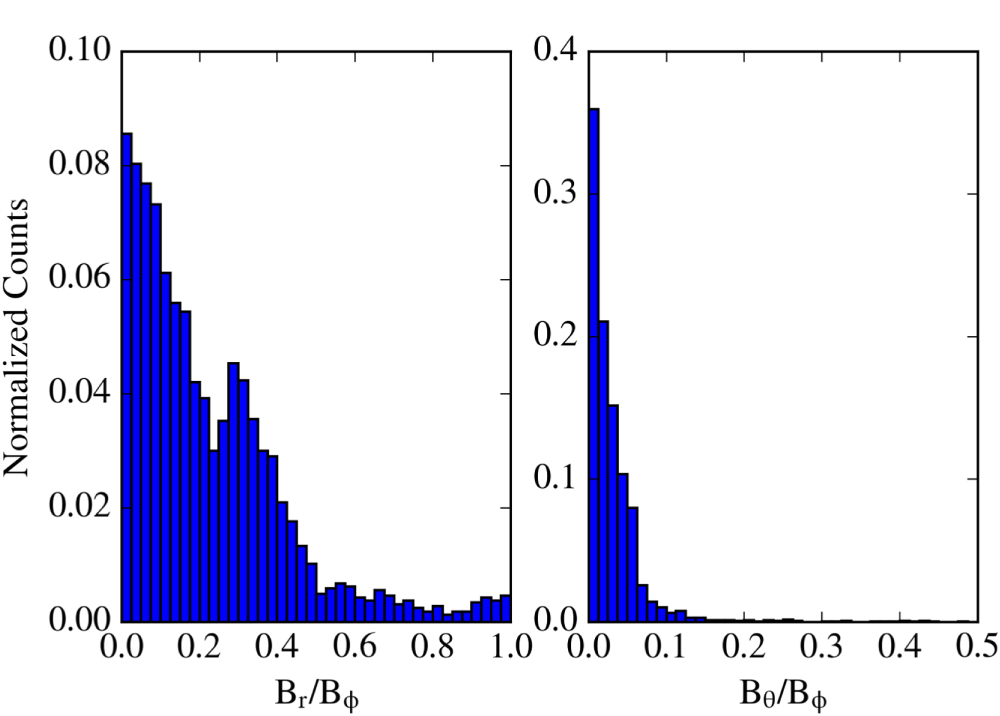
\includegraphics[width =\textwidth]{paper2_fig6.jpg}
	\caption{Histogram of guide fields in the SANE simulation, scaled to $B_{\phi}$, the component showing field reversal.  A large number of current sheets have no guide fields associated with them and, when present, the guide fields tend to be quite weak.}
	\label{SANE_bguide}
\end{figure}



The most promising subspace of this region for particle
acceleration to be efficient is the high-$\sigma$, low-$\beta$ (bottomright) regime, where there is maximal magnetic energy to
dissipate into the particles and fairly little gas pressure
relative to the magnetic pressure, such that the plasma is
magnetically dominated. The inferred ranges of $\sigma$ and $\beta$
are interesting for a number of reasons. Studies have only
recently begun for this transrelativistic regime (\citealt{werner2016})) and the physics of particle acceleration and
heating in these conditions are not yet fully understood.
While the ions in this regime remain non-relativistic (because $\sigma$ is of order 1), the electrons will likely be accelerated (or heated on average) to highly relativistic speeds,
since $\sigma_e \equiv B^2/(4\pi \rho_e c^2)=\sigma m_i/m_e \approx 10^3$, which is an
estimate of the characteristic electron Lorentz factors expected from reconnection.
Finally, in Figure \ref{SANE_bguide} we show a histogram of the relative guide field strengths in the SANE simulation. It is
evident that both cases of weak ($B_r/B_{\phi}] < 0.5$) and of no
guide fields are of interest for the purposes of these simulations. Even weak guide fields may play an important
and potentially adverse role in determining the outcome
of magnetic reconnection and must be explored via PIC simulations in the transrelativistic regime.

\subsection{Properties of MAD Current Sheets}

For the MAD simulation, we find that, in the regions of potential reconnection, $\sigma$ ranges from $10^{-3}$ to $10$, while $\beta$ ranges from $0.03$ to $10^{3}$ , as shown in Figure \ref{MAD_hist}. This is roughly an order of magnitude higher (lower) than the $\sigma$ ($\beta$) values in the SANE simulation, hinting that particle acceleration may be more efficient in these systems.

We show the guide fields in the MAD simulation in Figure \ref{MAD_bguide}. In stark contrast to the SANE guide fields, which are weak relative to the reconnecting field, the MAD guide fields are stronger and can be comparable to the reconnecting ones. While the typical values of the magnetization $\sigma$ and the plasma-$\beta$ are more favorable in terms of particle acceleration in the MAD simulations,
the stronger guide fields may alter the outcome of the reconnection event for the particle distribution.

\begin{figure}[!h]
	\centering
	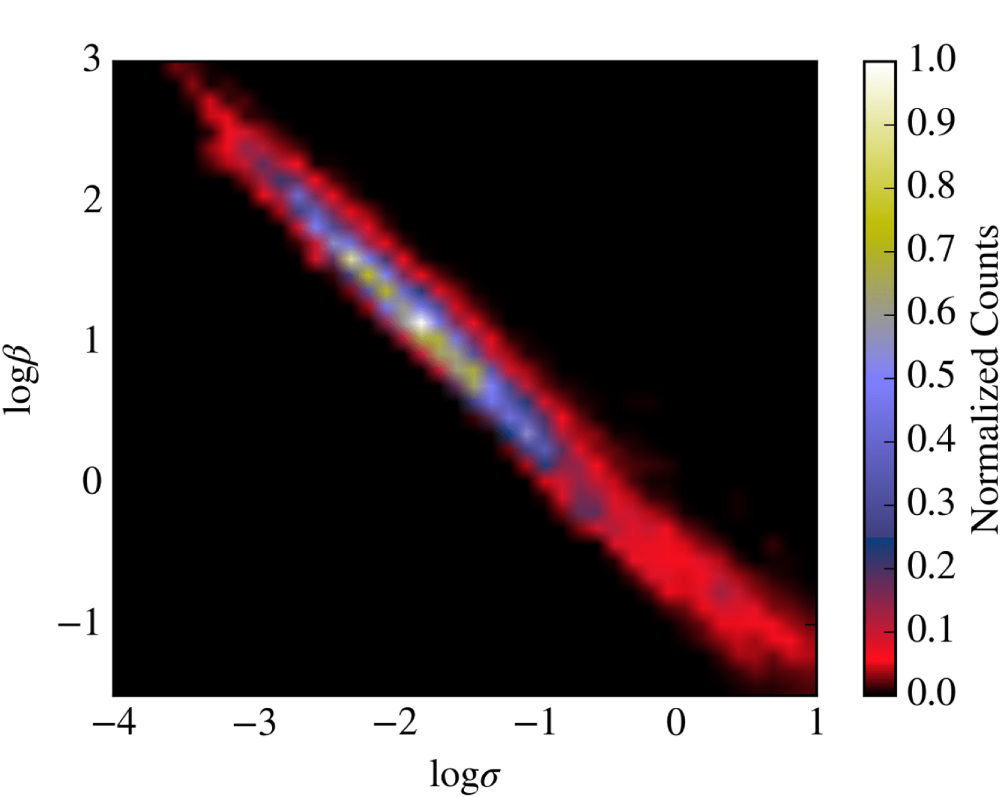
\includegraphics[width =\textwidth]{paper2_fig7.jpg}
	\caption{Two-dimensional histogram of the magnetization $\sigma$ and plasma-$\beta$ across all current sheets in the inner $10 \; GM/c^2$ of the MAD simulation.}
	\label{MAD_hist}
\end{figure}

\begin{figure}[!h]
	\centering
	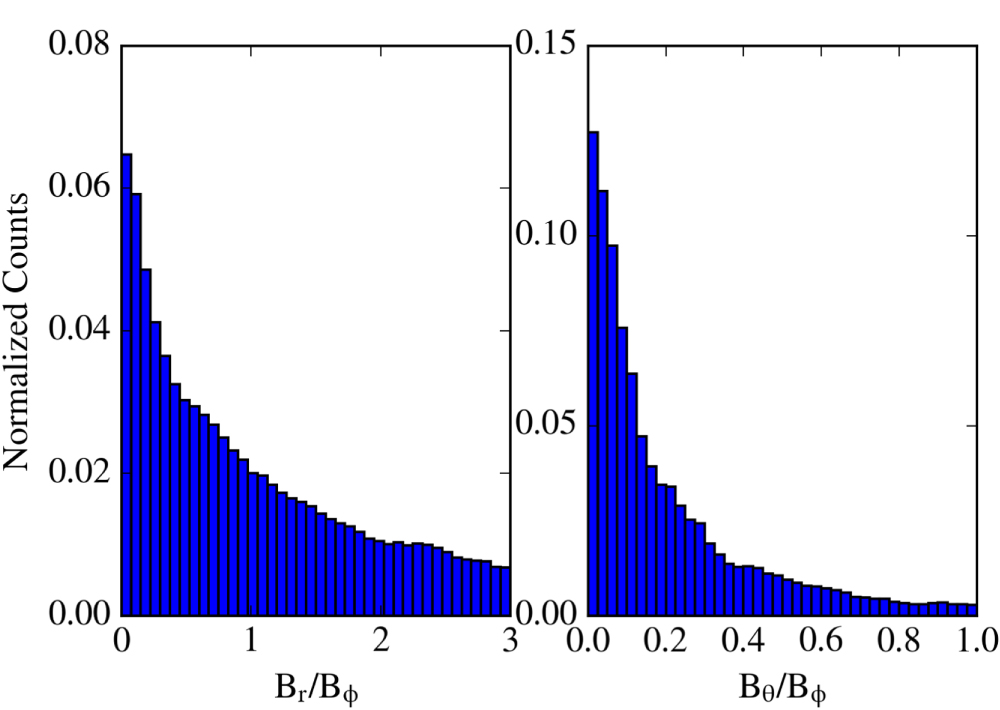
\includegraphics[width =\textwidth]{paper2_fig8.jpg}
	\caption{Histogram of guide fields in the MAD simulation, scaled to $B_{\phi}$, the component showing field reversal. While many sheets have little to no guide fields present, there are a significant number of current sheets with strong guide fields that will likely impact the efficiency of particle acceleration in these sheets.}
	\label{MAD_bguide}
\end{figure}


\section{Variability of Magnetic Energy available for Reconnection}

We finally examine the time variability of energy available to reconnection throughout the accretion flow. One
motivation for this is to assess whether reconnection
events can contribute substantially to the high energy
variability of low luminosity accretion flows, as has been
extensively observed in the case of Sgr A*. We integrate the magnetic energy density, $B^2/8\pi$, over the reconnecting volume bounded by the surfaces defined by
the asymptotic magnetic field location and obtain in this
way the total magnetic energy in the reconnection regions throughout the flow. We plot the results of this in
Figure 8 for both the SANE and MAD simulations.

\begin{figure*}[!h]
	\centering
	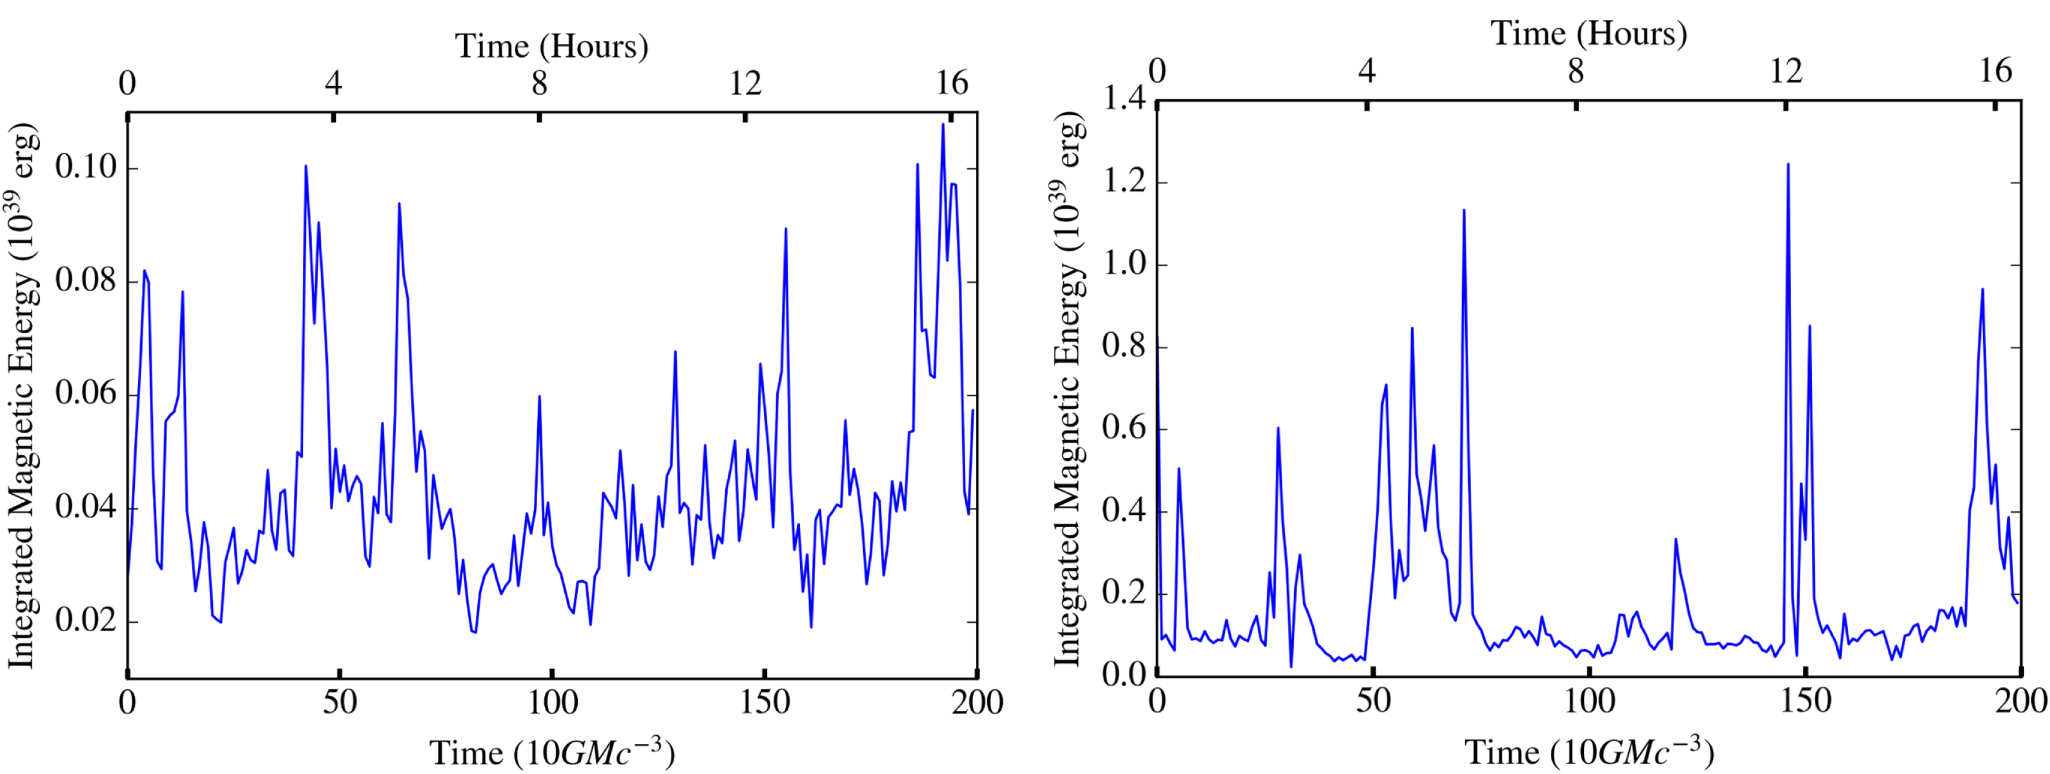
\includegraphics[width=\textwidth]{paper2_fig11.jpg}
	\caption{Magnetic energy of reconnection regions as a function of time in the (left) SANE and (right) MAD simulations. Note the rapid and strong variation over short timescales in both cases, making magnetic reconnection a promising candidate for contributing to the X-ray variability. }
	\label{mag_var}
\end{figure*}

We see that the turbulent nature of the accretion flow
very often leads to the formation of transient current
sheets that result in a highly time-varying magnetic energy being available to reconnection. This indicates that
magnetic reconnection likely is a significant contributor
to the variability of such systems. The SANE model
produces persistent variability due to the high levels of
turbulence in the disk. The MAD system has less turbulence and, hence, fewer variations, but the higher degree
of magnetization means that, when a current sheet does
develop, it typically has more magnetic energy associated
with it. For this reason, we find that the MAD simulation is characterized by fewer but stronger variations in the magnetic energy available to reconnection.

Figure \ref{sig_flare_hist} shows histograms of $\sigma$ for the current sheets of both SANE (left) and MAD (right) simulations, shown at a quiescent and flaring timestep. We see that during times of
increased magnetic energy, there tends to be an associated
population of current sheets with higher-than-typical magnetizations (around $\sigma \approx 1$ for the SANE case, and $\sigma \approx 10$ for MAD). This has significant implications for electron acceleration, because the typical energy of non-thermal electrons, as
well as the efficiency of electron acceleration both scale with $\sigma$.
\begin{figure}[!h]
	\centering
	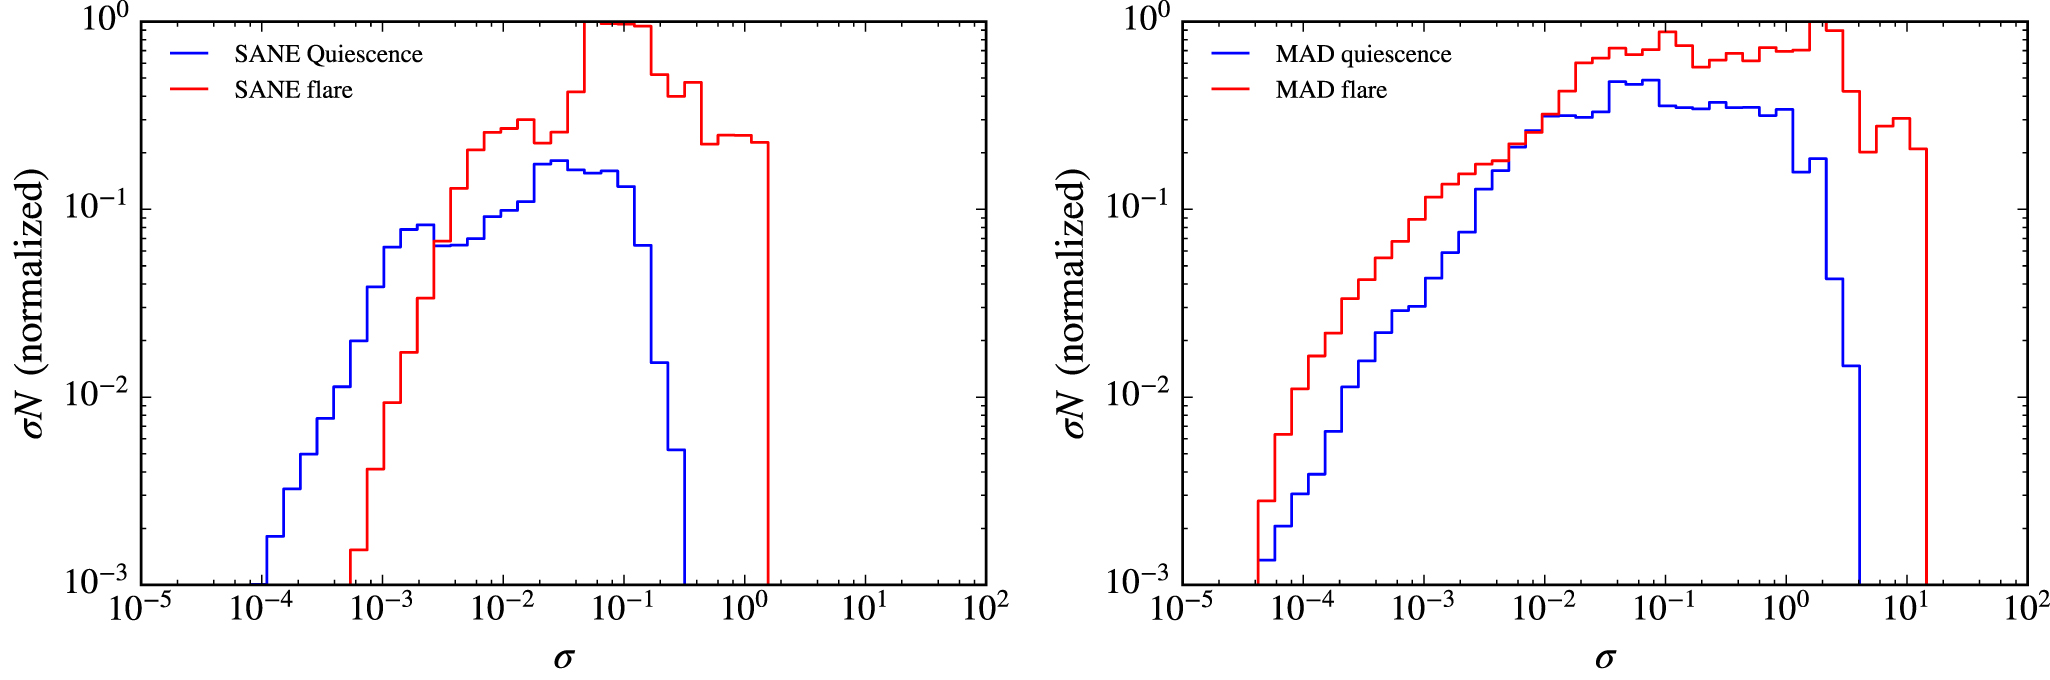
\includegraphics[width =\textwidth]{paper2_fig10.jpg}
	\caption{Histograms of $\sigma$ associated with current sheets in SANE (left) and MAD (right) simulations for both flaring and quiescent timesteps. We see that the increase in magnetic energy during a flaring time is associated with a population of current sheets with higher magnetizations.}
	\label{sig_flare_hist}
\end{figure}
Including the variability properties of non-thermal
electrons that are accelerated in these current sheets will
likely alter significantly the earlier finding of Chan et al.
(2015a), who used models that assumed a purely thermal electron distribution. In that early work, the variability of MAD simulations was characterized by smooth
long timescale variations in the flux. It is clear, however,
from the present analysis of the MAD simulation that
there is the potential for having a sudden injection of
non-thermal electrons associated with the spikes in Figure 5, which can then result in corresponding flares in
the lightcurve.
Based on previous studies, we expect some fraction of
this magnetic energy to go towards accelerating particles.
This acceleration efficiency will, in principle, depend on
the flow conditions, such as $\sigma$ and $\beta$, and can be found
through PIC simulations. In order to go from a picture
such as the one shown in Figure 8 to the non-thermal
particle energy as a function of time, the magnetic energy as a function of time must be combined with the
acceleration efficiency as a function of flow parameters,
which will likely result in even more dramatic variation
of energy on short timescales.
To estimate whether the energy available for reconnection is a plausible explanation for flares of these magnitudes, we calculate the total energy from an average X-ray flare from Sgr A*. Observations of X-ray flares from
Sgr A* show typical luminosities from  $\sim 10^{34}$ $\rm{erg} \rm{s}^{-1}$ to $2  10^{35} \; \rm{erg} \;  s^{-1}$ and typical timescales from hundreds of s to 8 ks (Neilsen et al. 2013). With a luminosity of $5 \times 10^{34} \; \rm{erg} \rm{s}^{-1}$ and a duration of 1000 s, about $5 \times 10^{37} \; \rm{erg}$ is being released in a typical flare.
Considering Figure 8, we see for the SANE model that
the energy available to reconnection peaks at typical values around $10^{38}$ erg, while typical MAD energies are an
order of magnitude higher than this. This shows that
there is enough energy available to reconnection in these
simulations to plausibly account for the observed energy
released during these flares. Moreover, the efficiency $\psi$
that determines the fraction of magnetic energy that goes
into particle acceleration must be quite high in the case
of SANE models, which have typically lower magnetizations and hence less magnetic energy associated with
their current sheets.
In Ball et al. (2016), we characterized the non-thermal
particle distribution using $\eta$, the fraction of non-thermal
to thermal energy densities in the fluid and power-law
index, p. We found that significant X-ray flares can occur
while satisfying the observed quiescent X-ray constraints
for values of $\eta = 0.1$ and a conservative power-law index
of $p = -3.5$. To connect our present results to these
earlier findings, we express $\eta$ in terms of $\beta$ and $\psi$ as
\begin{equation}
	\eta \equiv \frac{E_{nt}}{E_{th}}=\frac{\psi B^2}{nkT8\pi}=\psi \beta^{-1}.
\end{equation}
We can rewrite this as a constraint on the plasma-$\beta$ using the $\eta$ found in our previous study to result in significant X-ray variability, i.e., 
\begin{equation}
	0.1 (\frac{\eta}{0.1}) \beta \leq \psi.
\end{equation}
This places a constraint on the plasma-$\beta$, given a local
$\psi$, which must be found as a function of flow parameters
via PIC simulations. Note that $\psi$, by definition, cannot
be greater than 1, placing a strict upper limit of $\beta = 10$
for regions where there is sufficient magnetic energy to
accelerate particle to the energies required to generate
the flux excursions demonstrated in \citet{ball2016}.
More realistically, $\psi$ is likely to be of order 0.1, resulting
in an upper limit of $\beta \approx 1$. As shown in Figure \ref{label}, we find
that we indeed identify many current sheets satisfying
this condition.

\section{Conclusion}
In this paper, we investigated the detailed structure of
current sheets and their plasma properties in GRMHD
simulations of radiatively inefficient accretion flows. We
found that the regimes of plasma parameters relevant to
magnetic reconnection have been relatively unexplored
in terms of non-thermal particle acceleration. Specifically, we found that the magnetization $\sigma$ in the vicinity
of current sheets in the SANE simulation is of order $10^{-4}$
to $1$ , while the plasma-$\beta$ is of order $0.1$ to $10^3$
. Current sheets in the MAD simulation have magnetization
$\sigma$ ranging from $10^{-3}$
to $1$0 and plasma-$\beta$ from $0.03$ to
$10^3$. Additionally we find that, in these regions, there
is a relatively small spread in temperature, leading to a
tight correlation between the parameters $\sigma$ and $\beta$. We
also characterized the guide fields found in current sheets,
which can play a role in governing the details of particle
acceleration, and found that the ratio of guide field to
reconnecting field strength is typically 0–0.5 for SANE
simulations, but can be of order unity in MAD simulations.
GRMHD simulations need to use subgrid models in
order to account for physical effects that cannot be resolved or incorporated in MHD. In order to employ correctly subgrid models of reconnection, we must improve
our understanding of particle acceleration and heating in
the parameter space we lay out here.
In addition to characterizing the plasma properties of
current sheets, we also calculated the magnetic energy
available to reconnection throughout the simulations.
We found that the turbulent nature of the accretion flow
leads to current sheets of varying characteristics continuously forming and dissipating in the flow. This leads
to a highly variable amount of energy available to reconnect and dissipate into heating and particle acceleration
and makes magnetic reconnection a promising candidate
for contributing to the X-ray variability of Sgr A* and
other black holes with similar accretion characteristics.
Additionally, we found that there is indeed enough energy available to reconnection around current sheets to
account for typical flares observed from Sgr A*. We conclude that if this mechanism is responsible for the X-ray
flares, then the acceleration efficiency must be reasonably high for SANE disks and can be lower for the MAD
model.
